We present a series of experiments that illustrate the effect of using
the scheduling model and techniques discussed in the previous section.
These experiments focus on evaluating our techniques for managing the
overhead of transferring VM images to the nodes where they are
deployed.

Our experiments are divided into three sets:

\begin{description}
\item[\#1 Accuracy of AR deployments:] Investigates effect of scheduling image transfers on accuracy, using AR--only deployments. These experiments are run on our physical testbed, with our SGE--based implementation. A simulated experiment is also run to compare disk usage between the EDF and EDF/JIT image transfer algorithms.
\item[\#2 Efficiency in Best--effort deployments:] Investigates effect of image reuse in Best--effort deployments. These experiments are run on our physical testbed, with our SGE--based implementation.
\item[\#3 Mixing Best--effort and AR workloads:] Investigates what types of mixed workloads (Best--effort and AR) stand to benefit from using VMs, by using all off the techniques discussed in the previous sections. We focus on measuring the effect that virtualization has on utilization and running time of mixed workloads. These experiments are run using our simulator.
\end{description}

The physical testbed for experiments \#1 and \#2 is composed of 10 dual{}-CPU Pentium
III 500 MHz systems, each with 512 MB of RAM and 9G of local disk. One
node was used as a cluster head node, eight nodes for VM deployment,
and the remaining node as an image repository node, from which the VM
images would be transferred to the worker nodes. Nodes were connected
using 100 Mb/s switched Ethernet.

Virtual machine images were deployed using the SGE scheduler with the
extensions described in the previous section, based on traces that we developed for both
the advance reservation (AR) and best--effort cases. For the best--effort
cases, we used real workload traces, while for the AR cases, lacking
real AR submission workloads, we produced artificial traces using a
trace generator.

The simulated testbed for part of experiment \#1 and for experiment \#3 is also composed of 10 dual{}--CPU nodes, each with 1GB of memory, with eight worker nodes, one head node, and an image repository node. Nodes are connected using a 100 Mb/s switched Ethernet. We do not impose a limit on the local disk in each node, but keep track of how much disk space is used throughout the experiments, since the purpose of some of the experiments is precisely to show that disk usage can, in some cases, be excessive. The traces used in the simulations were artificially generated. The simulations were run on the University of Chicago's Department of Computer Science's Condor pool.

For all our experiments, we assumed that all virtual workspace requests
involved the same amount of CPU\% and memory for each virtual node. We
allowed at most 2 VMs to be deployed to a single physical node. Since
we focus on preparation overhead, the VW remains idle during its
runtime, and we assume that the VM generates no network traffic that
would share bandwidth with preparation overhead. This assumption is
reasonable in the case of highly parallel applications.

%The results from Experiments \#1 and \#2 (except the disk usage results from experiment \#1) were first presented in Sotomayor et al. \cite{overheadmatters}.

\section{Accuracy of AR deployments}

% Clarify that we are not using caching here.

Our first set of experiments investigates to what extent using
information on the relatively manageable overhead of VM scheduling can
improve the accuracy of providing a virtual resource to a
deadline{}-sensitive client. We assume that the client requests an advance reservation and we calculate accuracy (or
``client satisfaction'') as the ratio of the time the client actually
got to the requested time. Lacking any AR traces or existing AR trace generators,
we developed a simple trace generator capable of generating a large
number of requests according to a set of parameters. Since our SGE--based implementation does not support advance reservations, we then ran an
offline admission control algorithm on those requests to ensure that there exists a feasible
schedule for the submissions in the trace. Each submission represents
the deployment of a virtual cluster configured with the software
required to applications commonly run on the Open Science Grid (OSG),
and includes (1) the descriptor of the image template to use, (2) the
number of nodes, (3) the starting time of the workspace, and (4) its
duration. The Xen VM image with OSG worker node support that we used in
this experiment is 600 MB in size \cite{DBLP:conf/ccgrid/FosterFKSSZ06}. Nonetheless, we do not use any image reuse strategies in this experiment, as goal is to show that scheduling image transfers is, by itself, advantageous enough.

In this experiments we compare the EDF scheduling algorithm described in Section~\ref{cha:design} with non--scheduled file staging strategies. These strategies do not attempt to fit the image transfer in an optimal or near--optimal place in a schedule, but rather base the time of the image transfer directly on a fixed event, such as the submission time of a request or its starting time. The purpose of comparing against these strategies is to show that a scheduled approach not only guarantees accuracy, but it also better than easier--to--implement na\"ive strategies. In particular, we compare against the following (Figure~\ref{fig:filetransfer} summarizes these file staging strategies):

\begin{description}
\item[Job--style:]. The image transfer begins at the same time as the virtual resources, effectively invading it.
\item[Just In Time (JIT):] Assuming the network's full bandwidth is available for staging the necessary VM image for a workspace, the scheduler estimates the time required to transfer the image and starts the transfer before the start time, allocating just enough time to transfer the image.
\item[Aggressive:] This strategy attempts to transfer images immediately after the request has been accepted, regardless of the
starting time for the image transfer.
\end{description}



\begin{figure}
  \begin{center}
    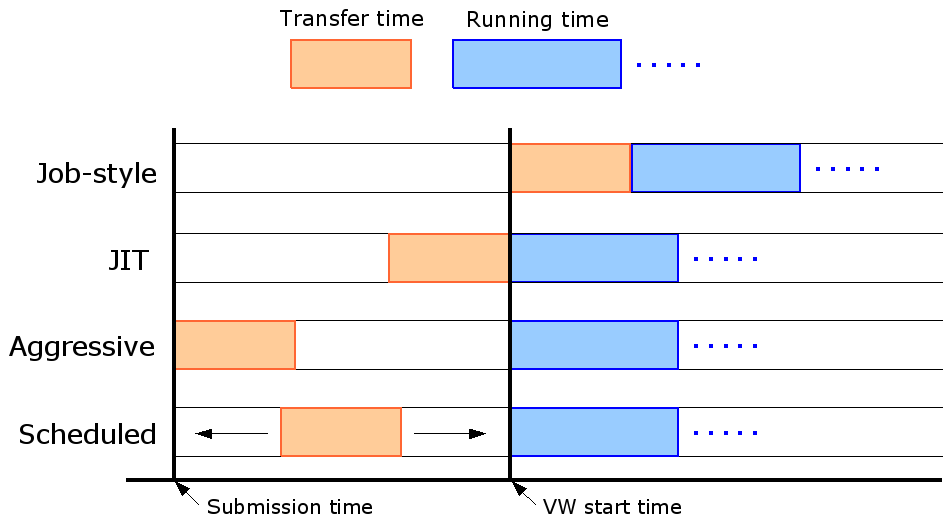
\includegraphics[width=0.8\textwidth]{figures/filetransfer.png}
    \caption{Naïve file staging strategies}
	\label{fig:filetransfer}
  \end{center}
\end{figure}


\newcolumntype{M}{>{\centering}m{0.15\textwidth}}
\newcolumntype{N}{>{\centering}m{0.3\textwidth}}

\begin{table}
\begin{center}
\begin{tabular}{|M|MM|MM|}

\cline{2-5}
\multicolumn{1}{M|}{}&
\multicolumn{1}{M|}{\bfseries Trace I}&
\multicolumn{1}{M|}{\bfseries Trace II}&
\multicolumn{1}{M|}{\bfseries Trace III}&
\multicolumn{1}{M|}{\bfseries Trace IV}

\\\hline

{\bfseries Trace duration (s)} &
\multicolumn{2}{N|}{7200}&
\multicolumn{2}{N|}{4700}

\\\hline

{\centering\bfseries \#~VW \nohyphens{submissions}} &
\multicolumn{1}{M|}{36}&
35 &
\multicolumn{2}{N|}{62}

\\\hline

{\bfseries Nodes per VW} &
\multicolumn{2}{N|}{2{}-4\newline (Uniformly distributed)} &
\multicolumn{2}{N|}{2{}-16\newline (Derived from original trace)}

\\\hline

{\bfseries Total images to deploy} &
\multicolumn{1}{M|}{110 (66.0GB)} &
{106\newline (63.6GB) } &
\multicolumn{2}{N|}{114 (86.4GB)}

\\\hline

{\bfseries VW Duration} &
\multicolumn{2}{N|}{1800s} &
\multicolumn{2}{N|}{Avg=53.0s\newline StDev=4.24s}

\\\hline

{\bfseries Starting times} &
\multicolumn{1}{M|}{Uniformly Distributed} &
{Clustered in 100s windows every 900s} &
\multicolumn{2}{N|}{\centering ASAP}

\\\hline

{\bfseries Images used} &
\multicolumn{2}{N|}{6 600MB images,\newline uniformly distributed} &
\multicolumn{2}{N|}{See Table 2}

\\\hline
\end{tabular}

\caption{Traces used in experiments}
\label{tab:traces}
\end{center}
\end{table}

Table~\ref{tab:traces} describes the two traces (I and II) used in this experiment.
These two traces differ in how the starting times of the VWs are
distributed throughout the duration of the experiment. In Trace I, the
starting times are distributed uniformly throughout the trace, while in
Trace II the starting times appear only during 100s windows (each
occurring every 900s), simulating VWs that are submitted in a bursty
fashion.

\begin{figure}
  \begin{center}
    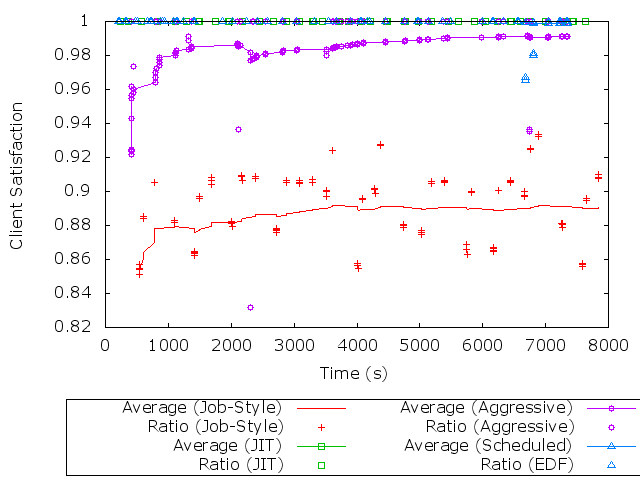
\includegraphics[width=0.8\textwidth]{figures/ClientSatisfaction-UniformStartTimes.png}
    \caption{Client Satisfaction (Trace I)}
	\label{fig:clientsatisfactionI}
  \end{center}
\end{figure}

Figure~\ref{fig:clientsatisfactionI} shows the results of running Trace I with the different image scheduling
strategies. We see that \emph{Scheduled} (EDF) and \emph{JIT} achieve 100\%
client satisfaction in most cases, followed by \emph{Aggressive} with
most submissions in the 96\%{}-100\% range. Since this trace represents
a best{}-case scenario, where the start times are uniformly distributed
throughout the experiment, even the na\"ive \emph{JIT} and
\emph{Aggressive} strategies achieve good performance.

\begin{figure}
  \begin{center}
    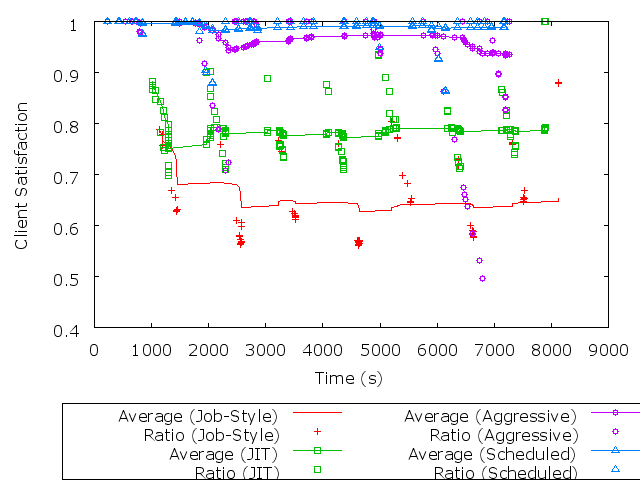
\includegraphics[width=0.8\textwidth]{figures/ClientSatisfaction-ClusteredStartTimes.png}
    \caption{Client Satisfaction (Trace II)}
	\label{fig:clientsatisfactionII}
  \end{center}
\end{figure}

Figure~\ref{fig:clientsatisfactionII} shows results with Trace II. Since \emph{JIT} allows just
enough time to transfer the image, regardless of what other VWs are
scheduled, this strategy can result in multiple image transfers being
scheduled during the same period of time (right before the ``window'').
As those transfers share available bandwidth, they take longer than
estimated. \emph{Scheduled} addressed this problem by prioritizing image
transfers and making use of network idle time, resulting in the best
performance, with few non{}-100\% satisfaction instances (and always at
the end of a ``window''). \emph{Aggressive}, on average, also has
good performance, but the images with tighter deadlines suffer as the
result of having to share bandwidth with other transfers.

\emph{Scheduled} is the only approach that
actually schedules a resource slot for the preparation overhead with
the goal of maximizing client satisfaction, while the other strategies
na\"ively start the image transfers at fixed times. By scheduling
overhead in the same way as virtual resources, instead of assuming that
overhead should be absorbed into the client's requested virtual
resource, \emph{Scheduled} achieves the best client satisfaction in the
two submission patterns present in traces I and II.

However, due to the limited disk space in our physical testbed, this setup is inadequate to observe how well disk usage scales. To do this, we use our simulator, running a trace of AR requests with the following characteristics:

\begin{itemize}
\item All ARs are known at the beginning of the trace.
\item Number of nodes per AR: 1--16 (uniformly distributed)
\item Number of requests: 94
\item Starting times: Uniformly distributed
\item Duration of trace: 10h
\end{itemize}

We compare the EDF and EDF/JIT image staging algorithms, and measure the peak disk usage in each node at each point in the experiment. Figure~\ref{fig:edfdiskusage} shows how EDF results in a high disk usage at the beginning of the experiment (as high as 31.2GB), since this algorithm will aggressively stage all the images to all the nodes as soon as possible. EDF/JIT, on the other hand, spreads the images transfers throughout the experiment, pushing the transfers as close as possible to the starting times of the reservations. This way, disk usage on any given node never exceeds 2.4GB (four images).

\begin{figure}
  \begin{center}
    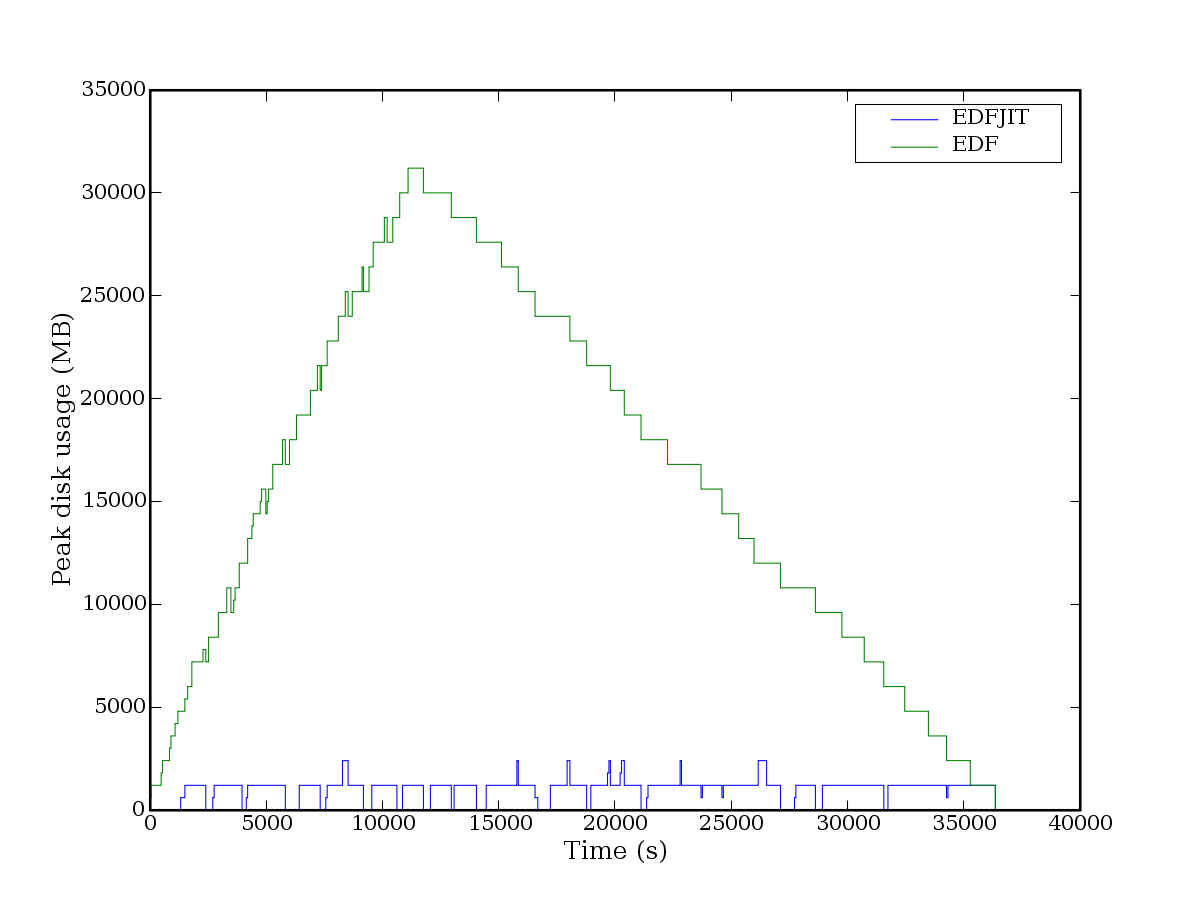
\includegraphics[width=0.8\textwidth]{figures/ar_edf.png}
    \caption{Disk usage with EDF and EDF/JIT}
	\label{fig:edfdiskusage}
  \end{center}
\end{figure}

\section{Efficiency in Best--effort deployments}

Our second set of experiments investigate two things: (1) how much in
terms of bandwidth usage the resource provider can save through
judicious use of image reuse based on workspace metadata and (2) to
what extent image reuse can improve deployment time (and thus also
client satisfaction) in situations where VM availability is requested
to start as soon as possible.

Since this experiment focuses on best--effort submissions, the same type of
submissions commonly found in batch systems, we were able to use a real
workload. In particular, we used the San Diego Supercomputer Center
(SDSC) DataStar log, available at the Parallel Workloads Archive \cite{BorjaCite21}.
We chose this workload because it explicitly distinguished submissions
for the DataStar's express queue (eight 8{}-CPU nodes, accepting jobs
lasting at most 2 hr), which allows us to test a scenario in which
minimizing deployment overhead is specially important: short{}-lasting
jobs. Since the SDSC DataStar log spans several months, we selected an
80 minute stretch of submissions (submissions \#21543 to \#21665 on
queue \#1) which we could run on our testbed. This extract was selected
because it represented a flurry of short{}-lasting jobs, which would
allow us to test how our system copes with the bandwidth requirements
of deploying a large amount of VM images.


\begin{table}
\begin{center}
\begin{tabular}{|c|c|c|c|c|}
\cline{2-5}
\multicolumn{1}{c|}{} &
\multicolumn{2}{c|}{\bfseries Trace III} &
\multicolumn{2}{c|}{\bfseries Trace IV}

\\\cline{2-5}

\multicolumn{1}{c|}{}  & {\bfseries Submissions} & {\bfseries Images} & {\bfseries Submissions} & {\bfseries Images} 

\\\hline

{\bfseries img.1} & 23\% & 21\% & 55\% & 60\%

\\\hline

{\bfseries img.2}
&
18\%
&
15\%
&
27\%
&
25\%

\\\hline

{\bfseries img.3}

&
15\%
&
12\%
&
6\%
&
6\%

\\\hline

{\bfseries img.4}
&
18\% 
&
15\%
&
5\%
&
4\%

\\\hline

{\bfseries img.5}
&
24\%
&
14\%
&
3\%
&
3\%

\\\hline

{\bfseries img.6}
&
3\%
&
12\%
&
3\%
&
3\%

\\\hline
\end{tabular}

\caption{Distribution of images in traces III, IV}
\label{tab:imagedistro}
\end{center}
\end{table}

When adapting the trace to our own experiments, each submission was
converted to a virtual cluster submission in which the number of nodes
was the number of requested processors in the original trace, scaled
down by four (the express queue has 64 processors; our testbed has 16),
with submission times and VW duration left unaltered. Each submission
was furnished with one of six 600 MB images. Two traces where produced,
with the only difference being the distribution of images assigned to
each submission. The first trace (Trace III) has images uniformly
distributed amongst the submissions, while in the second trace (Trace
IV) two images account for more than 80\% of the submissions. The
characteristics of theses traces are summarized in Table 1, while the
distribution of images is shown in Table~\ref{tab:imagedistro}. The rate at which VWs are
submitted is shown in Figure~\ref{fig:providershape}.

\begin{figure}
  \begin{center}
    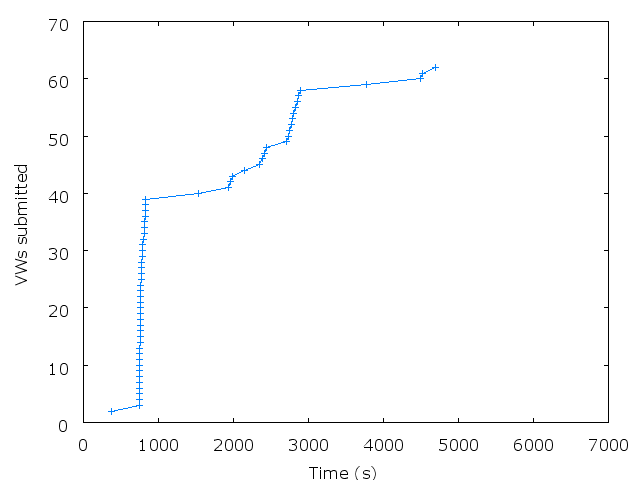
\includegraphics[width=0.8\textwidth]{figures/ProviderPerspective-TraceShape.png}
    \caption{VW Submissions (Traces III and IV)}
	\label{fig:providershape}
  \end{center}
\end{figure}

\begin{figure}
  \begin{center}
    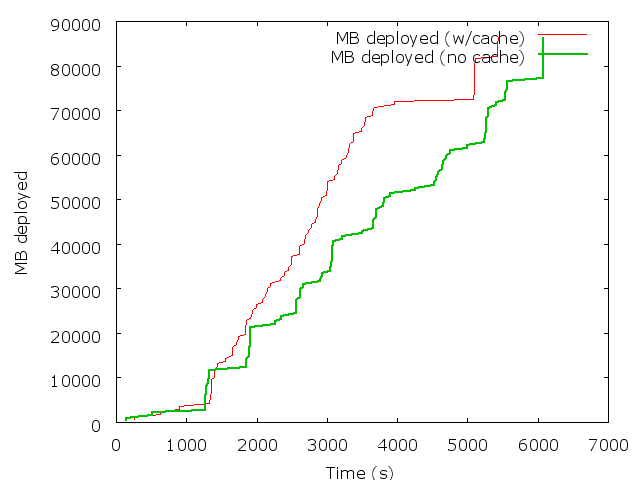
\includegraphics[width=0.8\textwidth]{figures/ProviderPerspective-Uniform2.png}
    \caption{MB Deployed (Trace III)}
	\label{fig:providerIII}
  \end{center}
\end{figure}

\begin{figure}
  \begin{center}
    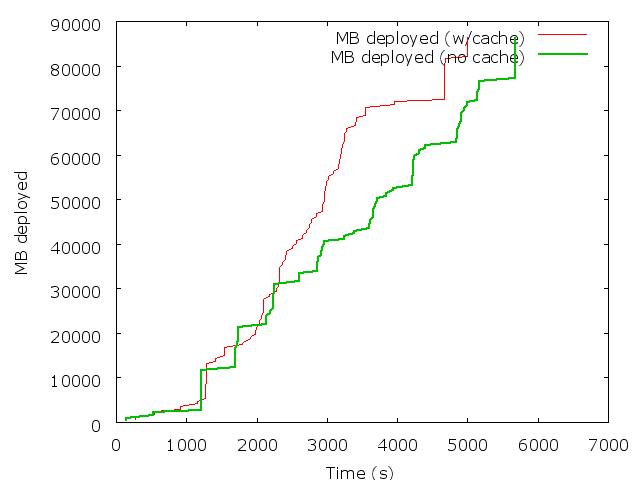
\includegraphics[width=0.8\textwidth]{figures/ProviderPerspective-Pareto2.png}
    \caption{MB Deployed (Trace IV)}
	\label{fig:providerIV}
  \end{center}
\end{figure}

Since these experiments use our SGE--based implementation, we used a 1.8 GB
LFU cache in each node (enough to cache three images) to minimize deployment time and increase throughput. The next set of experiments, run on our simulator, will present results using our image reuse algorithm.

Figure~\ref{fig:providerIII} shows
the cumulative number of MB transferred, overlaid with the VW
submissions. We can observe how, after the 2000s mark, the rate at
which images are deployed starts to increase, thanks to the reduced
transfer time resulting from the use of a cache. The difference in
effectively deployed MB is greatest at the 3550s mark, where the cached
approach results in a 25.2 GB ``advantage'' over the non{}-cached
approach. Figure~\ref{fig:providerIV}, shows the same data from running trace IV, where
the distribution of images favors a much larger number of cache hits.
Throughput is slightly better, with a difference of 27.6 GB at that
same 3550s mark.

Deployment time (not shown in graphs) is also improved. The average
deployment time for a single image, when not using a cache, is 440s for
both traces. This time is reduced to 305s and 247s, in Trace III and IV
respectively, when using an image cache.

These two experiments highlight how using the VW metadata to reuse image
templates and avoid redundant transfers benefits both the provider, by
offering a better utilization of resources leading to higher
throughput, and the consumer, by reducing the deployment time of best--effort
workspaces.


\section{Mixing Best--effort and AR workloads}

Our third set of experiments measures the effect of using our virtual resource model on workloads that combine both AR and best--effort requests. In particular, we are interested in finding under what conditions using VMs, with the techniques described in previous sections, could provide better performance. In particular, we measure the time to complete all best--effort requests and the utilization of physical resources.

We use several artificially--generated traces which mix best--effort requests and advance reservations. All these traces request enough resources such that, even with 100\% utilization throughout the experiment, each would require between 10h and 10.5h to complete. All ARs are known in advance by the scheduler (i.e., the requests are processed at the beginning of the trace), with starting times uniformly distributed throughout the experiment time. Best--effort requests arrive throughout the duration of the experiment, separated by uniformly separated intervals. 

We generate 36 different traces where we vary three parameters:

\begin{description}
\item[Proportion of Best--effort/AR requests:] This proportion is measured in terms of total running time requested by each type of request if they were run in sequence. For example, a workload with 10 advance reservations, each requesting two virtual nodes with a duration each of 5 minutes (total duration = $10\cdot 2\cdot 5$ = 100 minutes), and five best--effort requests, each requiring 10 virtual nodes with a duration each of 12 minutes (total duration = $5\cdot 10\cdot 12$ = 300 minutes), would be a proportion of 25\% AR and 75\% Best--effort. 

The purpose of this parameter is to observe what effect an increasing number of ARs can have on a Best--effort workload. We use the following proportions:
\begin{itemize}
\item 25\% Best--effort, 75\% AR
\item 50\% Best--effort, 50\% AR
\item 75\% Best--effort, 25\% AR
\end{itemize}
\item[Duration of best--effort requests:] A best--effort request will require $n$ virtual nodes, each running for time $t$, and scheduled serially (i.e., the nodes do not have to run in parallel). We explore different durations, to explore the effect on the backfilling and suspend/resume strategies (as described in Section~\ref{cha:design}, backfilling will be less effective in the presence of long--duration requests). We use the following durations:
\begin{itemize}
\item short: Average duration = 5 minutes
\item medium: Average duration = 10 minutes
\item long: Average duration = 15 minutes
\end{itemize}
It should be noted that, since we want the total duration of the workload to be ~10h, the value of $n$ will be inversely proportional to $t$. For example, if we reduce the duration of the best--effort requests, we must also increase the number of such requests. The actual value of $n$ will be determined by the proportion of Best--effort and AR requests. So, this parameter also allows us to observe what happens when the total number of best--effort requests in a trace increases (which will involve a larger number of image transfers).
\item[AR resource consumption:] This parameter controls how many physical resources are consumed by an AR request. This translates to how many virtual nodes are requested by an AR (a minimum of 1 and a maximum of 16, in our simulated testbed with 8 physical nodes, each with a capacity for 2 VMs). We explore the following values:
\begin{itemize}
\item Up to 25\% of available physical resources (1--4 nodes)
\item 25\% to 50\% (5--8 nodes)
\item 50\% to 75\% (9--12 nodes)
\item 75\% to 100\% (13--16 nodes)
\end{itemize}
\end{description}

Each request is assigned a VM image out of 37 possible 600MB images (22.2GB total). The distribution is skewed in such a way that seven images account for 70\% of requests (10\% each), and the remaining images account for 30\% of requests (1\% each). Since disk usage is one of our concerns, this distribution of images allows us to verify that our file prefetching and reusage strategies avoid accumulating all 37 images on the nodes. Furthermore, this is a case where predeployment of all the images might not be an acceptable solution (e.g., if we were dealing with 5GB images, that would mean using 185GB on each physical node), 

\subsection{Performance with predeployed VM images}

We start by running the traces in the following two configurations:

\begin{description}
\item[No virtualization] The time before an AR is backfilled (as described in Section~\ref{cha:design}), and there are no images to deploy.
\item[Virtualization, with predeployed images] Before an AR, best--effort requests are suspended and resumed after the AR (as described in Section~\ref{cha:design}, there are no images to deploy, and we assume a 10\% runtime overhead.
\end{description}

The purpose of comparing these two configurations is to observe what types of traces benefit the most from using the suspend/resume capabilities of virtual machines, despite the presence of runtime overhead, and under the assumption that image predeployment is acceptable. Table~\ref{tab:noVMvsPredeploy} shows time (in seconds) required to complete all the best--effort requests. Values in italics denote a case where using VMs results in better performance (shorter running time).

\begin{table}
\begin{center}
\begin{tabular}{|c|c|c|c|c|c|}
\hline
\textbf{Duration} & \textbf{AR resources} & \textbf{Batch-AR} & \textbf{(1)} & \textbf{(2)} & \textbf{$\frac{(2)}{(1)}$}
\\\hline
long & 000-025 & 25-75 & 38880 & 39000 & 0.309\%
\\\hline
long & 000-025 & 50-50 & 41160 & 41880 & 1.749\%
\\\hline
long & 000-025 & 75-25 & 41160 & 43500 & 5.685\%
\\\hline
long & 025-050 & 25-75 & 38400 & 37200 & \textcolor{blue}{\textit{-3.125}\%}
\\\hline
long & 025-050 & 50-50 & 41820 & 39360 & \textcolor{blue}{\textit{-5.882}\%}
\\\hline
long & 025-050 & 75-25 & 41100 & 42360 & 3.066\%
\\\hline
long & 050-075 & 25-75 & 37260 & 37020 & \textcolor{blue}{\textit{-0.644}\%}
\\\hline
long & 050-075 & 50-50 & 37320 & 37500 & 0.482\%
\\\hline
long & 050-075 & 75-25 & 42060 & 40080 & \textcolor{blue}{\textit{-4.708}\%}
\\\hline
long & 075-100 & 25-75 & 38700 & 37020 & \textcolor{blue}{\textit{-4.341}\%}
\\\hline
long & 075-100 & 50-50 & 41160 & 37260 & \textcolor{blue}{\textit{-9.475}\%}
\\\hline
long & 075-100 & 75-25 & 45780 & 42180 & \textcolor{blue}{\textit{-7.864}\%}
\\\hline
medium & 000-025 & 25-75 & 38700 & 39060 & 0.930\%
\\\hline
medium & 000-025 & 50-50 & 40800 & 42900 & 5.147\%
\\\hline
medium & 000-025 & 75-25 & 40140 & 43140 & 7.474\%
\\\hline
medium & 025-050 & 25-75 & 36840 & 36960 & 0.326\%
\\\hline
medium & 025-050 & 50-50 & 37200 & 37020 & \textcolor{blue}{\textit{-0.484}\%}
\\\hline
medium & 025-050 & 75-25 & 41220 & 42780 & 3.785\%
\\\hline
medium & 050-075 & 25-75 & 33420 & 33780 & 1.077\%
\\\hline
medium & 050-075 & 50-50 & 37260 & 36780 & \textcolor{blue}{\textit{-1.288}\%}
\\\hline
medium & 050-075 & 75-25 & 40800 & 41520 & 1.765\%
\\\hline
medium & 075-100 & 25-75 & 37380 & 36600 & \textcolor{blue}{\textit{-2.087}\%}
\\\hline
medium & 075-100 & 50-50 & 38640 & 37860 & \textcolor{blue}{\textit{-2.019}\%}
\\\hline
medium & 075-100 & 75-25 & 40800 & 40860 & 0.147\%
\\\hline
short & 000-025 & 25-75 & 36120 & 38700 & 7.143\%
\\\hline
short & 000-025 & 50-50 & 40860 & 43260 & 5.874\%
\\\hline
short & 000-025 & 75-25 & 41820 & 45240 & 8.178\%
\\\hline
short & 025-050 & 25-75 & 36600 & 36540 & \textcolor{blue}{\textit{-0.164}\%}
\\\hline
short & 025-050 & 50-50 & 40380 & 41340 & 2.377\%
\\\hline
short & 025-050 & 75-25 & 41160 & 43140 & 4.810\%
\\\hline
short & 050-075 & 25-75 & 30960 & 31020 & 0.194\%
\\\hline
short & 050-075 & 50-50 & 36900 & 37200 & 0.813\%
\\\hline
short & 050-075 & 75-25 & 39180 & 40980 & 4.594\%
\\\hline
short & 075-100 & 25-75 & 36600 & 36600 & 0.000\%
\\\hline
short & 075-100 & 50-50 & 37740 & 37560 & \textcolor{blue}{\textit{-0.477}\%}
\\\hline
short & 075-100 & 75-25 & 41040 & 42840 & 4.386\%
\\\hline
\end{tabular}

\textbf{(1)} No virtualization 
\textbf{(2)} Virtualization, with predeployed images
\caption{Effect of virtualization (assuming predeployed images) on time to complete best--effort requests}
\label{tab:noVMvsPredeploy}
\end{center}
\end{table}

We can observe the following in the results:
\begin{itemize}
\item The most noticeable performance gains occur in the presence of long best--effort requests. Since the time before an AR cannot be backfilled with shorter requests, using suspend/resume results in increased performance. In fact, the gain in performance is enough to overcome the runtime overhead of using VMs.
\item On the other hand, the presence of short best-effort requests allows the backfilling algorithm to achieve good enough performance in the non-VM case. In most cases, little is gained by using the suspend/resume capabilities of VMs (not enough to overcome the runtime overhead of VMs).
\end{itemize}

Table~\ref{tab:noVMvsPredeployUtil} compares both cases again, this time from the point of view of utilization. Utilization is measured as the percent of physical resources used (not idle) at a given time. In our case, since all requests require the same amount of CPU and memory, allowing for two VMs to run on the same machine, measuring CPU and memory would yield the same utilization percentage, so we simply record the percent of CPUs used at any given time. Table~\ref{tab:noVMvsPredeployUtil}, in particular, shows the average utilization at the end of the experiment. Since the 10\% runtime overhead results in higher utilization, the table makes a comparison assuming no runtime overhead. As in Table~\ref{tab:noVMvsPredeploy}

\begin{table}
\begin{center}
\begin{tabular}{|c|c|c|c|c|c|}
\hline
\textbf{Duration} & \textbf{AR resources} & \textbf{Batch-AR} & \textbf{(1)} & \textbf{(2)} & \textbf{$\frac{(2)}{(1)}$}
\\\hline
short & 000-025 & 25-75 & 0.87 & 0.86 & -0.45\%
\\\hline
short & 000-025 & 50-50 & 0.89 & 0.9 & 1.34\%
\\\hline
short & 000-025 & 75-25 & 0.9 & 0.91 & 0.72\%
\\\hline
short & 025-050 & 25-75 & 0.75 & 0.75 & 0.16\%
\\\hline
short & 025-050 & 50-50 & 0.89 & 0.92 & 3.22\%
\\\hline
short & 025-050 & 75-25 & 0.89 & 0.91 & 1.93\%
\\\hline
short & 050-075 & 25-75 & 0.61 & 0.61 & 0.00\%
\\\hline
short & 050-075 & 50-50 & 0.79 & 0.8 & 0.82\%
\\\hline
short & 050-075 & 75-25 & 0.87 & 0.89 & 2.19\%
\\\hline
short & 075-100 & 25-75 & 0.65 & 0.65 & 0.00\%
\\\hline
short & 075-100 & 50-50 & 0.83 & 0.86 & 3.11\%
\\\hline
short & 075-100 & 75-25 & 0.87 & 0.91 & 4.58\%
\\\hline
medium & 000-025 & 25-75 & 0.88 & 0.88 & 0.62\%
\\\hline
medium & 000-025 & 50-50 & 0.9 & 0.92 & 3.03\%
\\\hline
medium & 000-025 & 75-25 & 0.93 & 0.94 & 1.98\%
\\\hline
medium & 025-050 & 25-75 & 0.77 & 0.77 & 0.00\%
\\\hline
medium & 025-050 & 50-50 & 0.86 & 0.87 & 0.73\%
\\\hline
medium & 025-050 & 75-25 & 0.88 & 0.93 & 5.20\%
\\\hline
medium & 050-075 & 25-75 & 0.62 & 0.62 & 0.00\%
\\\hline
medium & 050-075 & 50-50 & 0.78 & 0.8 & 2.98\%
\\\hline
medium & 050-075 & 75-25 & 0.87 & 0.93 & 7.25\%
\\\hline
medium & 075-100 & 25-75 & 0.66 & 0.68 & 3.18\%
\\\hline
medium & 075-100 & 50-50 & 0.77 & 0.81 & 4.71\%
\\\hline
medium & 075-100 & 75-25 & 0.83 & 0.88 & 5.42\%
\\\hline
long & 000-025 & 25-75 & 0.85 & 0.85 & -0.37\%
\\\hline
long & 000-025 & 50-50 & 0.88 & 0.92 & 5.05\%
\\\hline
long & 000-025 & 75-25 & 0.91 & 0.94 & 3.15\%
\\\hline
long & 025-050 & 25-75 & 0.75 & 0.77 & 2.57\%
\\\hline
long & 025-050 & 50-50 & 0.82 & 0.92 & 12.05\%
\\\hline
long & 025-050 & 75-25 & 0.88 & 0.92 & 4.26\%
\\\hline
long & 050-075 & 25-75 & 0.62 & 0.62 & 0.57\%
\\\hline
long & 050-075 & 50-50 & 0.77 & 0.77 & 0.00\%
\\\hline
long & 050-075 & 75-25 & 0.83 & 0.91 & 9.35\%
\\\hline
long & 075-100 & 25-75 & 0.63 & 0.66 & 4.94\%
\\\hline
long & 075-100 & 50-50 & 0.74 & 0.84 & 12.62\%
\\\hline
long & 075-100 & 75-25 & 0.78 & 0.92 & 18.29\%
\\\hline
\end{tabular}

\textbf{(1)} No virtualization 
\textbf{(2)} Virtualization, with predeployed images
\caption{Effect of virtualization (assuming predeployed images) on utilization}
\label{tab:noVMvsPredeployUtil}
\end{center}
\end{table}

\subsection{Performance when VM images must be transferred}

The above predeployment results allow us to observe the effects of using suspend/resume without worrying about how preparation overhead factors into the results. Now we analyze what happens when VM images are not predeployed and must be transferred to the physical nodes before the VM can start. We compare the following configurations:

\begin{description}
\item[No virtualization.] Same as above.
\item[Virtualization, with predeployed images.] Same as above.
\item[Virtualization, with prefetching but no reuse.] Before an AR, best--effort requests are suspended and resumed after the AR, images are deployed using EDF/JIT for ARs, and FIFO for best--effort requests (as described in Section~\ref{cha:design}, and we assume a 10\% runtime overhead.
\item[Virtualization, with prefetching and reuse.] Same as previous, but using the image reuse algorithm described in Section~\ref{cha:design}
\end{description}

Table~\ref{tab:predeployVSfetch} shows the time to run all best--effort requests in the two virtualized configurations without predeployment, and compares them against the virtualized configuration with predeployment. This allows us to see what effect image prefetching and reuse have, and if they can achieve a performance as good as predeploying images. Values with an asterisk denote a case where image reuse results in a performance gain of more than 50\% compared to not using image reuse.

\begin{table}
\begin{center}
\begin{tabular}{|c|c|c|c|c|c|c|c|}
\hline
\textbf{Duration} & \textbf{AR resources} & \textbf{Batch-AR} & \textbf{(1)} & \textbf{(2)} & \textbf{(3)} &  \textbf{$\frac{(2)}{(1)}$} & \textbf{$\frac{(3)}{(1)}$}
\\\hline
long & 000-025 & 25-75 & 39000 & 39120 & 39120 & 0.31\% & 0.31\%
\\\hline
long & 000-025 & 50-50 & 41880 & 42180 & 41760 & 0.72\% & -0.29\%
\\\hline
long & 000-025 & 75-25 & 43500 & 44640 & 43920 & 2.62\% & 0.97\%
\\\hline
long & 025-050 & 25-75 & 37200 & 37380 & 37560 & 0.48\% & 0.97\%
\\\hline
long & 025-050 & 50-50 & 39360 & 40080 & 39420 & 1.83\% & 0.15\%
\\\hline
long & 025-050 & 75-25 & 42360 & 43260 & 42420 & 2.13\% & 0.14\%
\\\hline
long & 050-075 & 25-75 & 37020 & 37500 & 37140 & 1.30\% & 0.32\%
\\\hline
long & 050-075 & 50-50 & 37500 & 37680 & 37620 & 0.48\% & 0.32\%
\\\hline
long & 050-075 & 75-25 & 40080 & 41100 & 40140 & 2.55\% & 0.15\%
\\\hline
long & 075-100 & 25-75 & 37020 & 37320 & 37140 & 0.81\% & 0.32\%
\\\hline
long & 075-100 & 50-50 & 37260 & 37620 & 37440 & 0.97\% & 0.48\%
\\\hline
long & 075-100 & 75-25 & 42180 & 43500 & 42180 & 3.13\% & 0.00\%
\\\hline
medium & 000-025 & 25-75 & 39060 & 39060 & 39540 & 0.00\% & 1.23\%
\\\hline
medium & 000-025 & 50-50 & 42900 & 44040 & 42780 & 2.66\% & -0.28\%
\\\hline
medium & 000-025 & 75-25 & 43140 & 45660 & 42960 & 5.84\% & -0.42\%
\\\hline
medium & 025-050 & 25-75 & 36960 & 37200 & 37140 & 0.65\% & 0.49\%
\\\hline
medium & 025-050 & 50-50 & 37020 & 39540 & 37140 & 6.81\% & 0.32\%
\\\hline
medium & 025-050 & 75-25 & 42780 & 46740 & 42420 & 9.26\% & 0.84\%
\\\hline
medium & 050-075 & 25-75 & 33780 & 34380 & 33960 & 1.78\% & 0.53\%
\\\hline
medium & 050-075 & 50-50 & 36780 & 38580 & 36600 & 4.89\% & -0.49\%
\\\hline
medium & 050-075 & 75-25 & 41520 & 47040 & 41640 & 13.30\% & 0.29\%
\\\hline
medium & 075-100 & 25-75 & 36600 & 37680 & 36660 & 2.95\% & 0.16\%
\\\hline
medium & 075-100 & 50-50 & 37860 & 40980 & 38340 & 8.24\% & 1.27\%
\\\hline
medium & 075-100 & 75-25 & 40860 & 46080 & 41220 & 12.78\% & 0.88\%
\\\hline
short & 000-025 & 25-75 & 38700 & 40740 & 38820 & 5.27\% & 0.31\%
\\\hline
short & 000-025 & 50-50 & 43260 & 62580 & 45420 & 44.66\% & 4.99\%
\\\hline
short & 000-025 & 75-25 & 45240 & 81720 & 47040 & 80.64\% & 3.98\% \textcolor{green}{*}
\\\hline
short & 025-050 & 25-75 & 36540 & 38820 & 36840 & 6.24\% & 0.82\%
\\\hline
short & 025-050 & 50-50 & 41340 & 64320 & 42960 & 55.59\% & 3.92\% \textcolor{green}{*}
\\\hline
short & 025-050 & 75-25 & 43140 & 78180 & 46320 & 81.22\% & 7.37\% \textcolor{green}{*}
\\\hline
short & 050-075 & 25-75 & 31020 & 32220 & 32700 & 3.87\% & 5.42\%
\\\hline
short & 050-075 & 50-50 & 37200 & 57840 & 39900 & 55.48\% & 7.26\%
\\\hline
short & 050-075 & 75-25 & 40980 & 78600 & 43020 & 91.80\% & 4.98\% \textcolor{green}{*}
\\\hline
short & 075-100 & 25-75 & 36600 & 43020 & 36840 & 17.54\% & 0.66\%
\\\hline
short & 075-100 & 50-50 & 37560 & 64800 & 38700 & 72.52\% & 3.04\% \textcolor{green}{*}
\\\hline
short & 075-100 & 75-25 & 42840 & 84540 & 44940 & 97.34\% & 4.90\% \textcolor{green}{*}
\\\hline
\end{tabular}

\textbf{(1)} Virtualization, with predeployed images
\textbf{(2)} Virtualization, with prefetching but no reuse
\textbf{(3)} Virtualization, with prefetching and reuse
\caption{Effect of image prefetching and reuse on time to complete best--effort requests (compared with image predeployment)}
\label{tab:predeployVSfetch}
\end{center}
\end{table}

We can observe that not reusing images can have a considerable impact on performance when the workload contains many small requests, nearly doubling running time in some cases. This is due to the large amounts of images that must be transferred as part of the workload. On the other hand, the impact on performance gets smaller as the number of images to deploy decreases (with long requests, the impact on performance is only slightly larger that 3\% in the worst case).

Reusing images palliates, to a certain degree, the preparation overhead of the image transfers. While the improvement for long and medium requests is small, it is quite noticeable for short requests, where image reuse can bring performance considerably closer to that achieved when predeploying images. Considering that, without image reuse, performance is in some cases half as good as the predeployment case, it makes image reuse an appealing option for workloads where the number of image transfers require more than the available network bandwidth.

Table~\ref{tab:predeployVSfetchUtil} is similar to Table~\ref{tab:predeployVSfetch}, but shows the effect on utilization. In this table, we can observe that utilization is affected in the same way as the running time of the best--effort requests. Table~\ref{tab:novmVSfetch} compares the virtualized configurations against the non-virtualized configuration.

Finally, disk usage was measured in all these experiments. When using VMs, with images prefetched with EDF/JIT, disk usage on the physical nodes never exceeded 3.6GB (six images). When using the reuse algorithm, disk usage was slightly smaller, peaking at 3.0GB (five images). We also ran the experiments using the EDF image transfer algorithm and, similarly to the results in the `Accuracy of AR deployments' experiments, disk usage was much higher, peaking at 30GB (50 images).

\begin{table}
\begin{center}
\begin{tabular}{|c|c|c|c|c|c|c|c|}
\hline
\textbf{Duration} & \textbf{AR resources} & \textbf{Batch-AR} & \textbf{(1)} & \textbf{(2)} & \textbf{(3)} &  \textbf{$\frac{(2)}{(1)}$} & \textbf{$\frac{(3)}{(1)}$}
\\\hline
long & 000-025 & 25-75 & 0.92 & 0.91 & 0.91 & -0.36\% & -0.29\%
\\\hline
long & 000-025 & 50-50 & 0.93 & 0.92 & 0.93 & -0.84\% & 0.18\%
\\\hline
long & 000-025 & 75-25 & 0.94 & 0.92 & 0.93 & -2.71\% & -0.99\%
\\\hline
long & 025-050 & 25-75 & 0.78 & 0.78 & 0.78 & -0.40\% & -0.84\%
\\\hline
long & 025-050 & 50-50 & 0.94 & 0.92 & 0.93 & -1.75\% & -0.14\%
\\\hline
long & 025-050 & 75-25 & 0.94 & 0.92 & 0.94 & -2.08\% & -0.09\%
\\\hline
long & 050-075 & 25-75 & 0.67 & 0.66 & 0.66 & -1.32\% & -0.30\%
\\\hline
long & 050-075 & 50-50 & 0.83 & 0.83 & 0.83 & -0.40\% & -0.27\%
\\\hline
long & 050-075 & 75-25 & 0.94 & 0.92 & 0.94 & -2.59\% & -0.16\%
\\\hline
long & 075-100 & 25-75 & 0.72 & 0.71 & 0.71 & -0.78\% & -0.38\%
\\\hline
long & 075-100 & 50-50 & 0.89 & 0.88 & 0.89 & -0.94\% & -0.43\%
\\\hline
long & 075-100 & 75-25 & 0.93 & 0.9 & 0.93 & -3.20\% & -0.04\%
\\\hline
medium & 000-025 & 25-75 & 0.9 & 0.9 & 0.89 & 0.03\% & -1.22\%
\\\hline
medium & 000-025 & 50-50 & 0.94 & 0.91 & 0.94 & -2.63\% & 0.27\%
\\\hline
medium & 000-025 & 75-25 & 0.95 & 0.89 & 0.95 & -5.84\% & 0.32\%
\\\hline
medium & 025-050 & 25-75 & 0.79 & 0.78 & 0.79 & -0.68\% & -0.41\%
\\\hline
medium & 025-050 & 50-50 & 0.94 & 0.88 & 0.93 & -6.70\% & -0.32\%
\\\hline
medium & 025-050 & 75-25 & 0.93 & 0.85 & 0.94 & -9.23\% & 0.84\%
\\\hline
medium & 050-075 & 25-75 & 0.64 & 0.64 & 0.64 & 0.00\% & 0.00\%
\\\hline
medium & 050-075 & 50-50 & 0.85 & 0.81 & 0.85 & -4.92\% & 0.52\%
\\\hline
medium & 050-075 & 75-25 & 0.93 & 0.83 & 0.93 & -13.16\% & -0.26\%
\\\hline
medium & 075-100 & 25-75 & 0.73 & 0.71 & 0.72 & -2.92\% & -0.22\%
\\\hline
medium & 075-100 & 50-50 & 0.87 & 0.8 & 0.86 & -8.32\% & -1.29\%
\\\hline
medium & 075-100 & 75-25 & 0.9 & 0.8 & 0.89 & -12.64\% & -0.76\%
\\\hline
short & 000-025 & 25-75 & 0.93 & 0.88 & 0.93 & -5.30\% & -0.28\%
\\\hline
short & 000-025 & 50-50 & 0.93 & 0.64 & 0.88 & -44.55\% & -4.94\%
\\\hline
short & 000-025 & 75-25 & 0.92 & 0.51 & 0.88 & -80.67\% & -3.98\%
\\\hline
short & 025-050 & 25-75 & 0.81 & 0.76 & 0.8 & -6.35\% & -0.79\%
\\\hline
short & 025-050 & 50-50 & 0.93 & 0.6 & 0.89 & -55.60\% & -4.04\%
\\\hline
short & 025-050 & 75-25 & 0.94 & 0.52 & 0.87 & -81.13\% & -7.38\%
\\\hline
short & 050-075 & 25-75 & 0.66 & 0.66 & 0.66 & 0.00\% & 0.00\%
\\\hline
short & 050-075 & 50-50 & 0.86 & 0.55 & 0.8 & -55.42\% & -7.17\%
\\\hline
short & 050-075 & 75-25 & 0.91 & 0.48 & 0.87 & -91.67\% & -4.98\%
\\\hline
short & 075-100 & 25-75 & 0.69 & 0.59 & 0.68 & -17.49\% & -0.57\%
\\\hline
short & 075-100 & 50-50 & 0.9 & 0.52 & 0.88 & -72.28\% & -2.90\%
\\\hline
short & 075-100 & 75-25 & 0.91 & 0.46 & 0.87 & -97.32\% & -4.99\%
\\\hline
\end{tabular}

\textbf{(1)} Virtualization, with predeployed images
\textbf{(2)} Virtualization, with prefetching but no reuse
\textbf{(3)} Virtualization, with prefetching and reuse
\caption{Effect of image prefetching and reuse on utilization (compared with image predeployment)}
\label{tab:predeployVSfetchUtil}
\end{center}
\end{table}



\begin{table}

\begin{center}
\begin{tabular}{|c|c|c|c|c|c|c|c|}
\hline
\textbf{Duration} & \textbf{AR resources} & \textbf{Batch-AR} & \textbf{(1)} & \textbf{(2)} & \textbf{(3)} &  \textbf{$\frac{(2)}{(1)}$} & \textbf{$\frac{(3)}{(1)}$}
\\\hline
long & 000-025 & 25-75 & 38880 & 39120 & 39120 & 0.62\% & 0.62\%
\\\hline
long & 000-025 & 50-50 & 41160 & 42180 & 41760 & 2.48\% & 1.46\%
\\\hline
long & 000-025 & 75-25 & 41160 & 44640 & 43920 & 8.46\% & 6.71\%
\\\hline
long & 025-050 & 25-75 & 38400 & 37380 & 37560 & \textcolor{blue}{\textit{-2.66\%}} & \textcolor{blue}{\textit{-2.19\%}}
\\\hline
long & 025-050 & 50-50 & 41820 & 40080 & 39420 & \textcolor{blue}{\textit{-4.16\%}} & \textcolor{blue}{\textit{-5.74\%}}
\\\hline
long & 025-050 & 75-25 & 41100 & 43260 & 42420 & 5.26\% & 3.21\%
\\\hline
long & 050-075 & 25-75 & 37260 & 37500 & 37140 & 0.64\% & \textcolor{blue}{\textit{0.32\%}}
\\\hline
long & 050-075 & 50-50 & 37320 & 37680 & 37620 & 0.97\% & 0.80\%
\\\hline
long & 050-075 & 75-25 & 42060 & 41100 & 40140 & \textcolor{blue}{\textit{-2.28\%}} & \textcolor{blue}{\textit{-4.57\%}}
\\\hline
long & 075-100 & 25-75 & 38700 & 37320 & 37140 & \textcolor{blue}{\textit{-3.57\%}} & \textcolor{blue}{\textit{-4.03\%}}
\\\hline
long & 075-100 & 50-50 & 41160 & 37620 & 37440 & \textcolor{blue}{\textit{-8.60\%}} & \textcolor{blue}{\textit{-9.04\%}}
\\\hline
long & 075-100 & 75-25 & 45780 & 43500 & 42180 & \textcolor{blue}{\textit{4.98\%}} & \textcolor{blue}{\textit{7.86\%}}
\\\hline
medium & 000-025 & 25-75 & 38700 & 39060 & 39540 & 0.93\% & 2.17\%
\\\hline
medium & 000-025 & 50-50 & 40800 & 44040 & 42780 & 7.94\% & 4.85\%
\\\hline
medium & 000-025 & 75-25 & 40140 & 45660 & 42960 & 13.75\% & 7.03\%
\\\hline
medium & 025-050 & 25-75 & 36840 & 37200 & 37140 & 0.98\% & 0.81\%
\\\hline
medium & 025-050 & 50-50 & 37200 & 39540 & 37140 & 6.29\% & \textcolor{blue}{\textit{-0.16\%}}
\\\hline
medium & 025-050 & 75-25 & 41220 & 46740 & 42420 & 13.39\% & 2.91\%
\\\hline
medium & 050-075 & 25-75 & 33420 & 34380 & 33960 & 2.87\% & 1.62\%
\\\hline
medium & 050-075 & 50-50 & 37260 & 38580 & 36600 & 3.54\% & \textcolor{blue}{\textit{-1.77\%}}
\\\hline
medium & 050-075 & 75-25 & 40800 & 47040 & 41640 & 15.29\% & 2.06\%
\\\hline
medium & 075-100 & 25-75 & 37380 & 37680 & 36660 & 0.80\% & \textcolor{blue}{\textit{-1.93\%}}
\\\hline
medium & 075-100 & 50-50 & 38640 & 40980 & 38340 & 6.06\% & \textcolor{blue}{\textit{-0.78\%}}
\\\hline
medium & 075-100 & 75-25 & 40800 & 46080 & 41220 & 12.94\% & 1.03\%
\\\hline
short & 000-025 & 25-75 & 36120 & 40740 & 38820 & 12.79\% & 7.48\%
\\\hline
short & 000-025 & 50-50 & 40860 & 62580 & 45420 & 53.16\% & 11.16\%
\\\hline
short & 000-025 & 75-25 & 41820 & 81720 & 47040 & 95.41\% & 12.48\% 
\\\hline
short & 025-050 & 25-75 & 36600 & 38820 & 36840 & 6.07\% & 0.66\%
\\\hline
short & 025-050 & 50-50 & 40380 & 64320 & 42960 & 59.29\% & 6.39\%
\\\hline
short & 025-050 & 75-25 & 41160 & 78180 & 46320 & 89.94\% & 12.54\%
\\\hline
short & 050-075 & 25-75 & 30960 & 32220 & 32700 & 4.07\% & 5.62\%
\\\hline
short & 050-075 & 50-50 & 36900 & 57840 & 39900 & 56.75\% & 8.13\% 
\\\hline
short & 050-075 & 75-25 & 39180 & 78600 & 43020 & 100.61\% & 9.80\% 
\\\hline
short & 075-100 & 25-75 & 36600 & 43020 & 36840 & 17.54\% & 0.66\%
\\\hline
short & 075-100 & 50-50 & 37740 & 64800 & 38700 & 71.70\% & 2.54\% 
\\\hline
short & 075-100 & 75-25 & 41040 & 84540 & 44940 & 105.99\% & 9.50\% 
\\\hline
\end{tabular}

\textbf{(1)} No virtualization
\textbf{(2)} Virtualization, with prefetching but no reuse
\textbf{(3)} Virtualization, with prefetching and reuse
\caption{Effect of image prefetching and reuse on time to complete best--effort requests (compared with no virtualization)}
\label{tab:novmVSfetch}
\end{center}
\end{table}



